\documentclass[a4paper,11pt]{article}
\usepackage[czech]{babel}
\usepackage[left=2cm,text={17cm,24cm},top=3cm]{geometry}
\usepackage[hidelinks]{hyperref}
\usepackage[utf8]{inputenc}
\usepackage[T1]{fontenc}
\usepackage[perpage]{footmisc}
\usepackage{graphicx}

\graphicspath{ {./resources/} }


\title{Dokumentace k projektu z IMP \\
        \large Měření vzdálenosti ultrazvukovým senzorem}

\author{Hung Do \\ \href{mailto:xdohun00@stud.fit.vutbr.cz}{xdohun00@stud.fit.vutbr.cz}}

\begin{document}
    \maketitle
    \thispagestyle{empty}
    \newpage
    \tableofcontents
    \newpage
    \section{Popis problému}
    Cílem tohoto projektu je za pomocí ultrazvukového senzoru HY-SRF05 naměřit vzdálenost a výslednou hodnotu zobrazit na 
    sedmi-segmentovým LED displeji. Oba senzor i displej musí být připojeny na vývojovou desku s mikrokontrolerem typu ARM.
    V tomto projektu byla použita vývojová deska FITkit v3.0. Všechny součástky byly zapůjčeny z Ústavu počítačových systémů (UPSY) na 
    Fakultě informačních technologií VUT v Brně.

    \section{Zapojení HW}
    \label{sec:circuit_diagram}
    \begin{figure}[ht!]
        \centering
        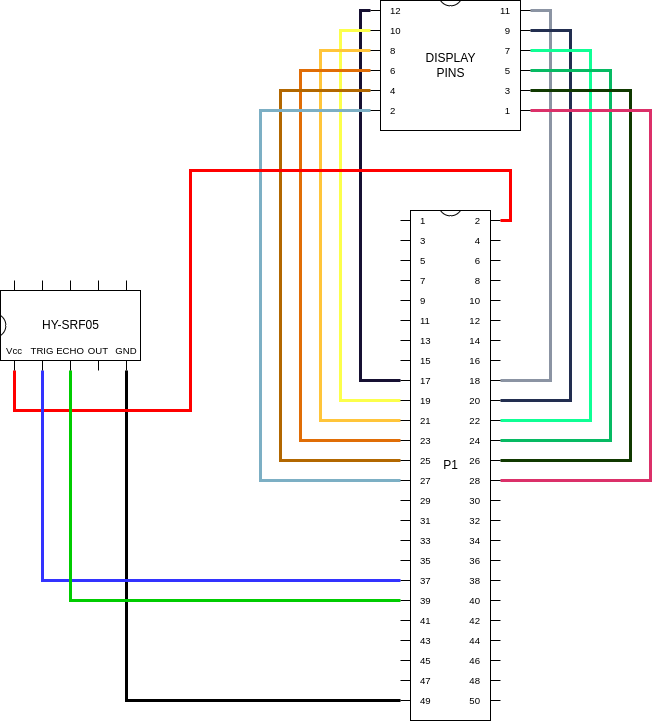
\includegraphics[width=280pt]{circuit}
        \caption{Zapojení systému}
    \end{figure}

    \section{Implementace}
    \subsection{Hlavní program}
    Program nejprve nainicializuje modul časovače a potřebné porty pro komunikaci se senzory. Ze zapojení \ref{sec:circuit_diagram} můžeme vidět,
    že ultrazvukový senzor i sedmi-segmentový displej jsou zapojený na programovatelných GPIO pinech portů \textbf{A} a \textbf{D}.
    Následně se inicializuje časový modul \textbf{PIT}, ve kterém se aktivují tři ze čtych kanálů. První kanál slouží k odpočtu 10 $\mu$s
    při generování signálu \emph{TRIG}. Druhý kanál uchovává délku pulzu mezi nástupnou a sestupnout hranou signálu \emph{ECHO}. Výsledek pak slouží
    k samotnému výpočtu vzdálenosti. A poslední třetí kanál opožďuje čas mezi jednotlivými měřěními (o 100 ms).

    V hlavní funkci programu se zapne signál \emph{TRIG} společně s prvním časovačem a následně se program přesune do
    nekonečné smyčky, ve které aktualizuje/zobrazuje vypočítanou vzdálenost na displeji.

    \subsection{Práce se segmentovým displejem}
    Program zobrazuje na displeji hodnotu uloženou v globální proměnné \verb|distance|. Hodnota je poté rozdělena na jednotlivé cifry a ty
    se postupně rozsvítí s určitým časovým zpožděním. Na zápis jednotlivých cifer byla naimplementovaná makra \verb|DIGIT_n(c_pos)|, kde \verb|n|
    určuje hodnota cifry a \verb|c_pos| určuje pozici na displeji.

    \subsection{Práce se ultrazvukovým senzorem}
    Celá práce s ultrazvukovým senzorem je řízená přes \textbf{PIT} modul a portem \textbf{A}. Nejprve je vygenerovaný signál \emph{TRIG} po dobu 10 $\mu$s,
    poté se čeká na nástupnou hranu signálu \emph{ECHO}. Po přijetí tohoto signálu se zapne \textbf{PIT1} časovač, který se zastaví až po přijetí
    sestupné hrany. Počet taktů se pak převedou na uběhnutý čas v $\mu$s a hodnota se vydělí číslem 58\footnote{viz. dokumentace \url{https://www.robot-electronics.co.uk/htm/srf05tech.htm}}.
    Výsledek je uložen do globální proměnné \verb|distance|.

    Paralelně s tímto jede třetí časovač \textbf{PIT2}, který po vypršení časového limitu opět vygeneruje \emph{TRIG} signál a měřění začne znovu.

    \subsection{Diagramy}
    \begin{figure}[ht!]
        \centering
        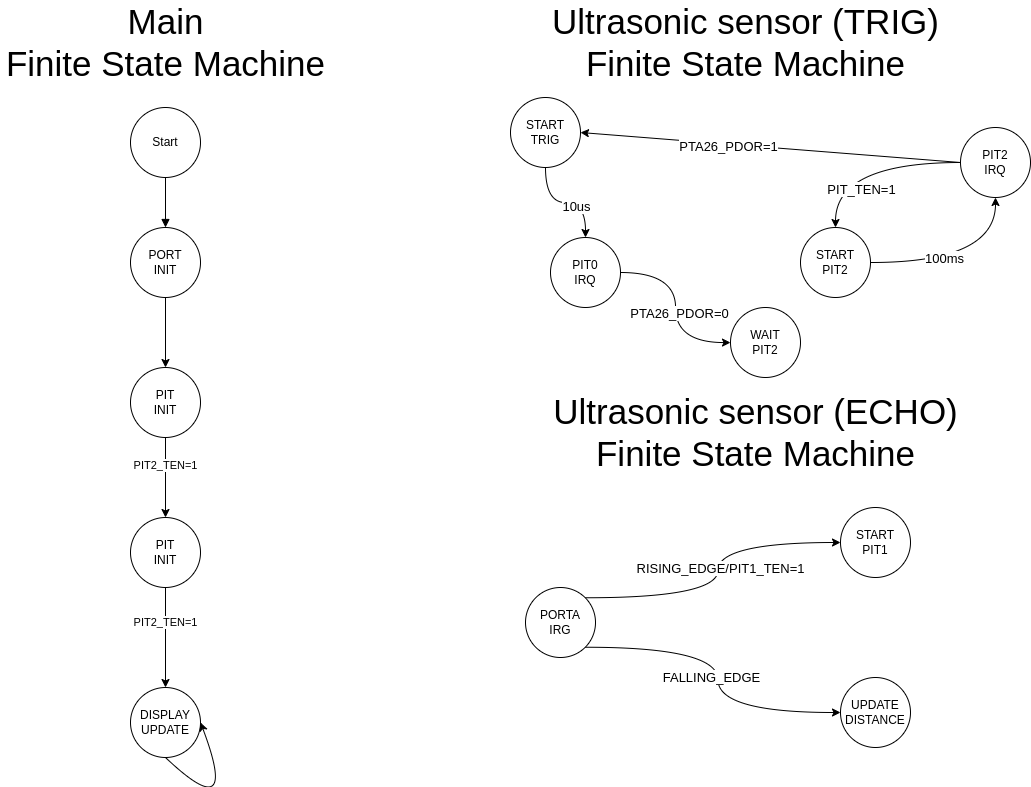
\includegraphics[width=450pt]{FSM}
        \caption{Konečný automat systému}
    \end{figure}
    \begin{figure}[ht!]
        \centering
        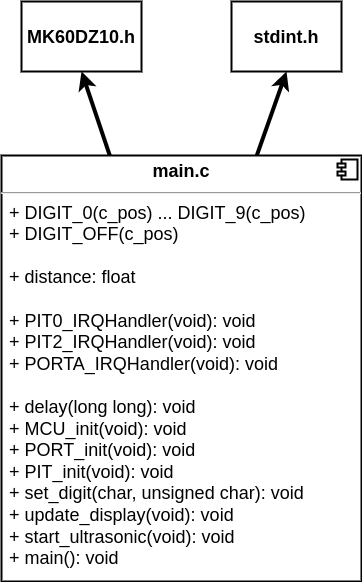
\includegraphics[width=150pt]{program}
        \caption{Struktura programu}
    \end{figure}
    \newpage

    \section{Závěr}
    Během testování senzor z nějakého neznámého důvodu vracel nižší hodnotu než se očekávalo. Například pro 16 cm senzor naměřil pouhých 13 cm.
    Prvním pokusem o zpřesnění výpočtu bylo změnou konstanty pro výpočet vzdálenosti z 58 na 50. Po této úpravě došlo k zlepšení výstupních hodnot.
    Nakonec bylo zapotřebí zinicializovat časový modul \textbf{MCG}, který nastavil frekvenci procesoru a poté již senzor měřil dobře (s konstantou 58).
    
    Při implementaci projektu bylo problémové též rozjetí displeje z důvodu rozmístění \emph{GPIO} portů na periferii \textbf{P1}.
    Šest pinů bylo umístěné na portu \textbf{A} a druhá polovina na portu \textbf{D}. Jinak byl projekt vcelku velice jednoduchý a zábavný. 

    \section{Doplňující odkazy}
    Odkaz na video: \url{https://drive.google.com/file/d/1qnb5OsGO1FpfHTN3c1mjMN9AdAEpws3M/view?usp=share_link}

\end{document}
